\documentclass[a4paper, notitlepage]{report}
\begin{titlepage}

\begin{center}

%% Insert the TU Delft logo at the bottom of the page.
\begin{tikzpicture}[remember picture,overlay]
    \node at (current page.south)[anchor=south,inner sep=0pt]{
        
\includegraphics{cover/logo}
    };
\end{tikzpicture}

%% Extra whitespace at the top.
\vspace*{2\bigskipamount}

%% Print the title in cyan.
{\makeatletter
\titlestyle\color{tudelft-cyan}\Huge\@title
\makeatother}

%% Print the optional subtitle in black.
{\makeatletter
\ifx\@subtitle\undefined\else
    \bigskip
    \titlefont\titleshape\LARGE\@subtitle
\fi
\makeatother}

\bigskip
\bigskip

by
%door

\bigskip
\bigskip

%% Print the name of the author.
{\makeatletter
\titlefont\Large\bfseries\@author
\makeatother}

\vfill

in partial fulfillment of the requirements for the degree of
%in overeenstemming met de vereisten voor het verkrijgen van de graad van

\bigskip
\bigskip

{\bfseries Master of Science}

in Applied Physics

\bigskip
\bigskip

at the Delft University of Technology,
%aan de Technische Universiteit Delft,

to be defended publicly on Tuesday January 1, 2013 at 10:00 AM.
%in het openbaar de verdedigen op dinsdag 1 januari om 10:00 uur.

\vfill

\begin{tabular}{lll}
%% Add additional information here, per faculty requirements, e.g
%    Student number: & 1234567 \\
%    Project duration: & \multicolumn{2}{l}{March 1, 2012 -- January 1, 2013} \\
    Supervisor: & Prof.\ dr.\ ir.\ A.\ Einstein \\
    Thesis committee:
        & Prof.\ dr.\ C.\ F.\ Xavier, & TU Delft \\
        & Dr.\ E.\ L.\ Brown, & TU Delft \\
        & Ir.\ M.\ Scott, & Acme Corporation
\end{tabular}

%% Only include the following lines if confidentiality is applicable.
\bigskip
\bigskip
\emph{This thesis is confidential and cannot be made public until December 31, 2013.}
%\emph{Op dit verslag is geheimhouding van toepassing tot en met 31 december 2013.}

\bigskip
\bigskip
An electronic version of this thesis is available at \url{http://repository.tudelft.nl/}.
%Een elektronische versie van dit verslag is beschikbaar op \url{http://repository.tudelft.nl/}.

\end{center}

\end{titlepage}


% All imports needed for file

% General
\usepackage[a4paper,top=1.25in,right=1in,bottom=1.25in,left=1in]{geometry}
\usepackage[utf8]{inputenc}
\usepackage[T1]{fontenc}
\usepackage{textcomp}
\usepackage[bitstream-charter]{mathdesign}
\usepackage{cite}

\usepackage{import}
\usepackage{standalone}
\usepackage{epstopdf}



% Math
\usepackage{amsmath}	% some standard math functions
%\usepackage{amssymb}	% more mathematical symbols
\usepackage{amsbsy}	% enable bold mathematics
\usepackage{bm}
%\usepackage{amsthm}	% enable theorem statements
\usepackage{trfsigns} 	% symbols for transforms

% Text formatting
\usepackage{fancyhdr}	% allow more control over page headers/footers
\usepackage{enumitem}	% allow control over enumerate, itemize, description
\usepackage{setspace}	% allow control over spacing
\usepackage{lastpage}	% provide label for last page in document
\usepackage{sectsty}	% allow control over section styling
\usepackage{url}

% Floats
\usepackage{xcolor}		% enable use of colors
\usepackage{graphicx}		% enable graphics
\usepackage{float}		% enable floats
\usepackage[section]{placeins}	% prevent floats from moving past e.g. sections
\usepackage[small, bf, hang, figurename=Fig.]{caption}	% enable captions for floats (images etc.)
\captionsetup{width=.8\textwidth} % captions not too wide
\usepackage{subcaption}		% enable subcaptions for floats (images etc.)
\usepackage[nottoc]{tocbibind}		% put more stuff in TOC

% Styling data
\pagestyle{fancyplain}

% Title page
\makeatletter
\let\inserttitle\@title
\makeatother

% Page header
\setlength{\headwidth}{\textwidth}
\lhead{} % leave left header empty
\chead{}
\rhead{} % leave right header empty
\lfoot{} % leave left footer empty
\cfoot{} % leave center footer empty
\rfoot{}
\renewcommand{\headrulewidth}{0.3pt}
\renewcommand{\footrulewidth}{0pt}

% Section, equation and figure numbering
\usepackage{chngcntr} 
\counterwithout{figure}{chapter}
\renewcommand{\thechapter}{\Roman{chapter}}
\renewcommand{\thesection}{\Roman{chapter}.\arabic{section}}
\renewcommand{\thesubsection}{\Roman{chapter}.\arabic{section}.\arabic{subsection}}
\renewcommand{\thesubsubsection}{\alph{subsubsection})}
\renewcommand{\thefigure}{\arabic{figure}}
\renewcommand{\thesubfigure}{\alph{subfigure}}
\renewcommand{\theequation}{\thechapter--\arabic{equation}}
\setcounter{tocdepth}{1}
\captionsetup[figure]{labelsep=period}

% Nice enumerations
\newlist{enum}{enumerate}{1}
\setlist[enum]{label=\textbf{[\arabic*]}} % \arabic or \alpha
\setlist{itemsep=-5pt}

% Nice \begin{StateDescription} for FSM descriptions
\newlist{StateDescription}{description}{1}
\setlist[StateDescription]{font=\normalfont\scshape, labelwidth=12em, leftmargin=12em,listparindent=0em,itemindent=0em}

% Section formatting
\definecolor{title-gray}{gray}{0.45}		% grijstint voor headers
\renewcommand*\sfdefault{lmss}
\allsectionsfont{\sffamily\color{title-gray}}	% sans-serif in headers

% Page layout
\onehalfspacing					% Wide margins for text
\usepackage{chngpage}			% customize margins of certain pages
\usepackage{adjustbox}

% Text macros
\usepackage{xspace}
\newcommand{\matlab}{MATLAB\xspace}		% fancy MATLAB command
\newcommand{\norm}[1]{\left\lVert#1\right\rVert}% Command for vector norm
\newcommand{\abs}[1]{\left\lvert#1\right\rvert}% Command for abs
\newcommand{\todo}[1]{\textbf{\textcolor{red}{#1}}}	% placeholder stuff
\let\oldhat\hat
\renewcommand{\vec}[1]{\bm{#1}} % bold vectors in math mode
\newcommand{\vechat}[1]{\oldhat{\bm{#1}}} % hat in vector mode
\newcommand{\mat}[1]{\bm{#1}} % bold matrix in math mode

%links
\usepackage{hyperref}
\hypersetup{ %setup hyperlinks
    colorlinks=true,
    citecolor=black,
    filecolor=black,
    linkcolor=black,
    urlcolor=black
}

\begin{document}

\section{Problem formulation}
\label{sec:sro-problem}
Two distinct aspects of the received signal samples require synchronization. The first is a fixed time offset between received signals, caused by to network lag and latency in handling the commands sent from the central computer. The second is due to frequency deviations from the intended sampling rate between different analog-to-digital converters.

\begin{figure}[hbt]
\begin{adjustwidth}{-1in}{-1in}
\centering
	\begin{subfigure}{0.25\paperwidth}
		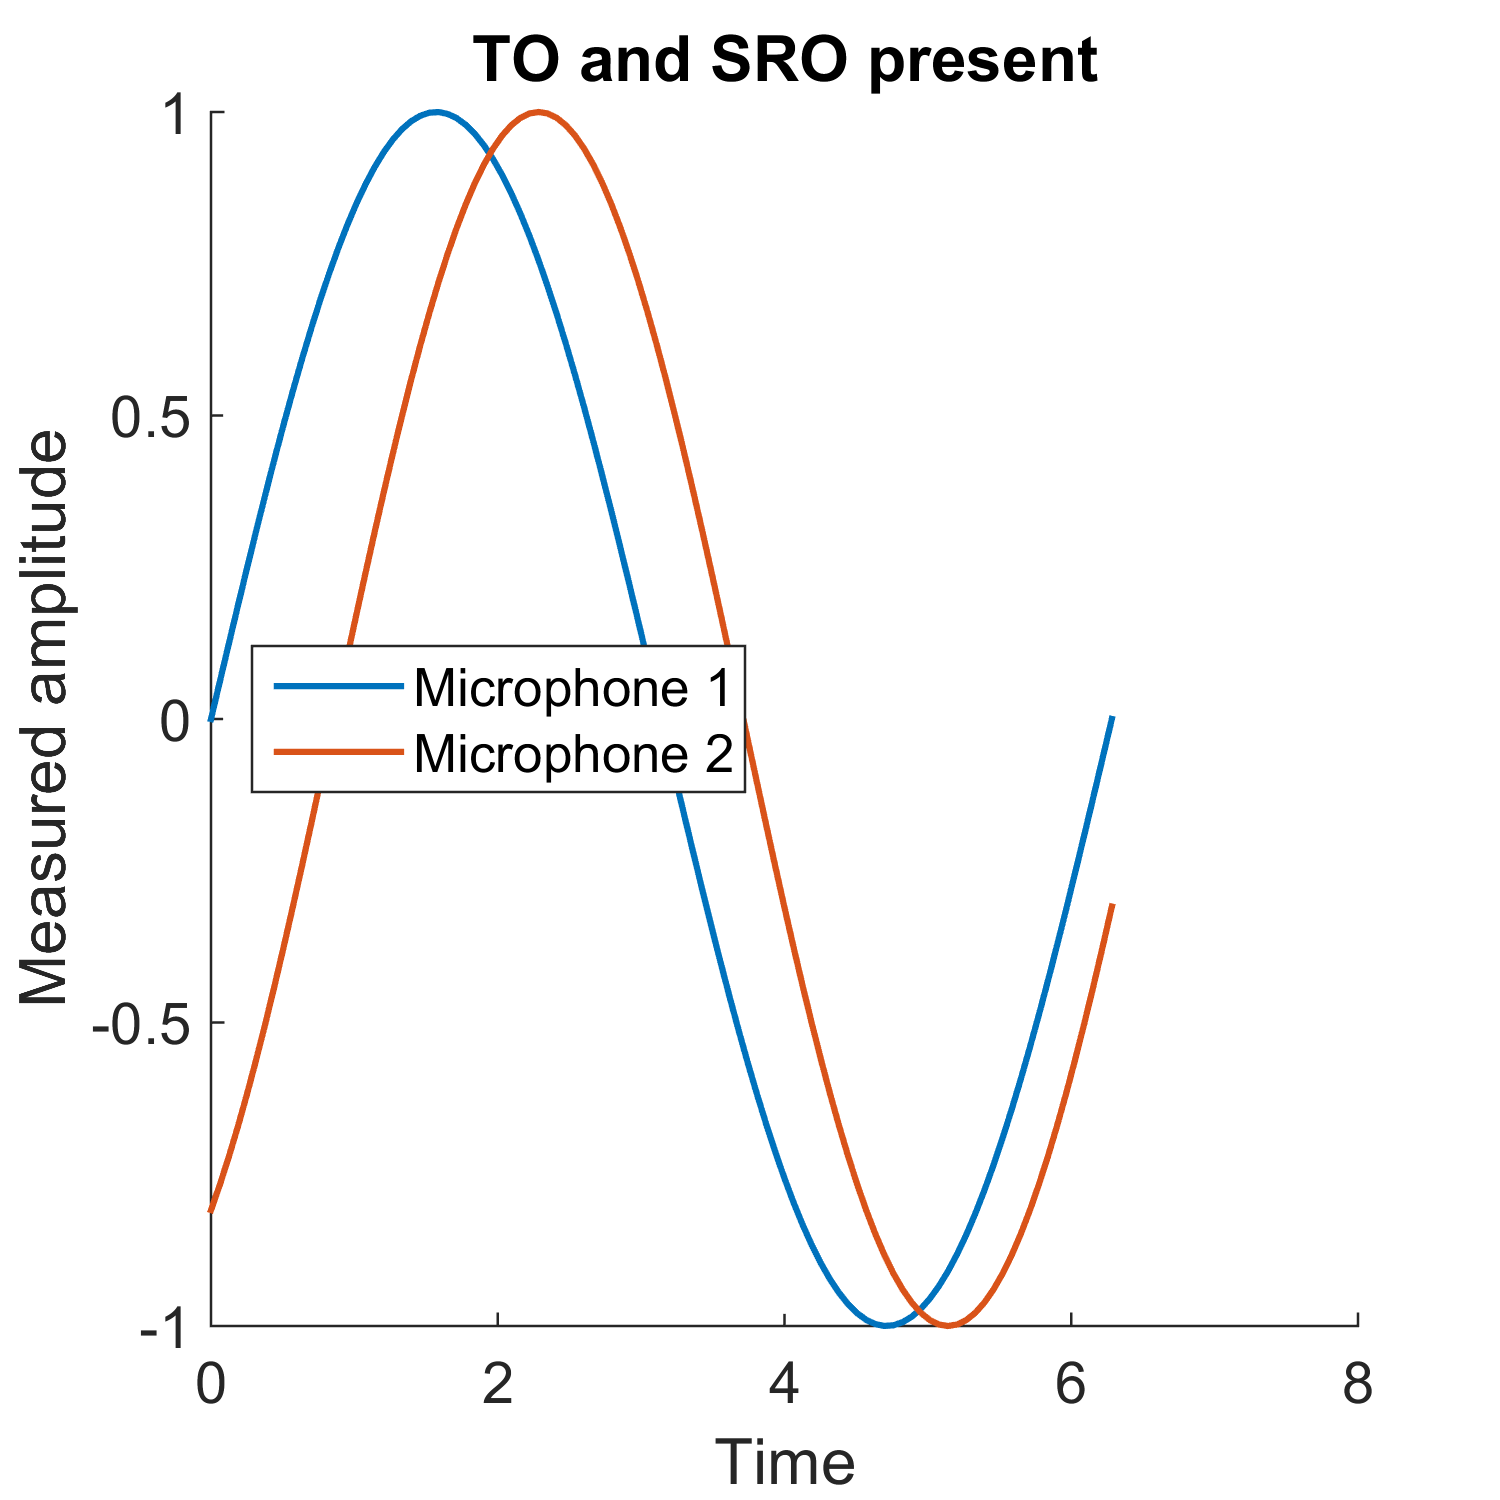
\includegraphics[width=\textwidth]{figures/sro-example/to-and-sro}
		\caption{Both TO and SRO are present in the measured microphone samples.}
		\label{fig:sync-ex1}
	\end{subfigure}
	~
	\begin{subfigure}{0.25\paperwidth}
		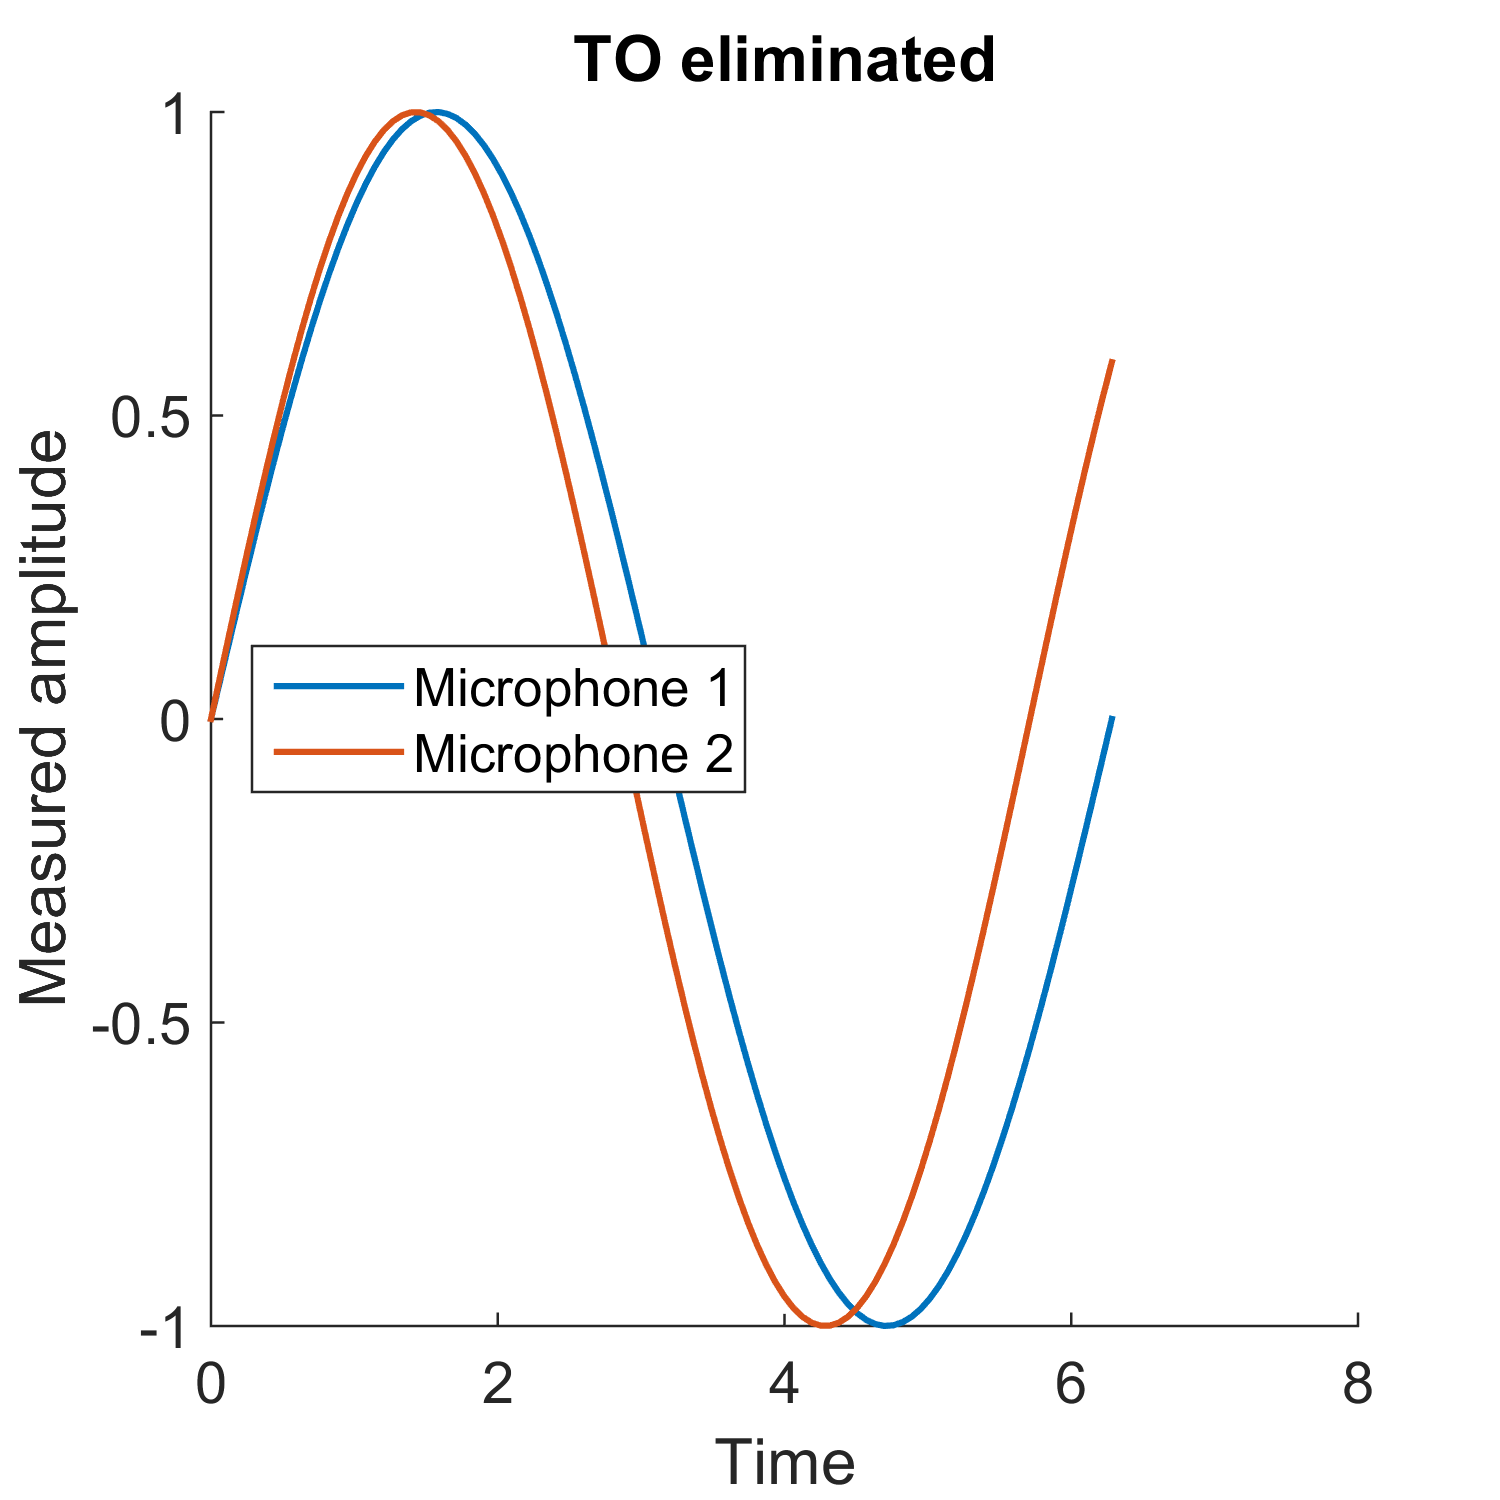
\includegraphics[width=\textwidth]{figures/sro-example/only-sro}
		\caption{TO eliminated, SRO is still present.}
		\label{fig:sync-ex2}
	\end{subfigure}
	
	
	\begin{subfigure}{0.25\paperwidth}
		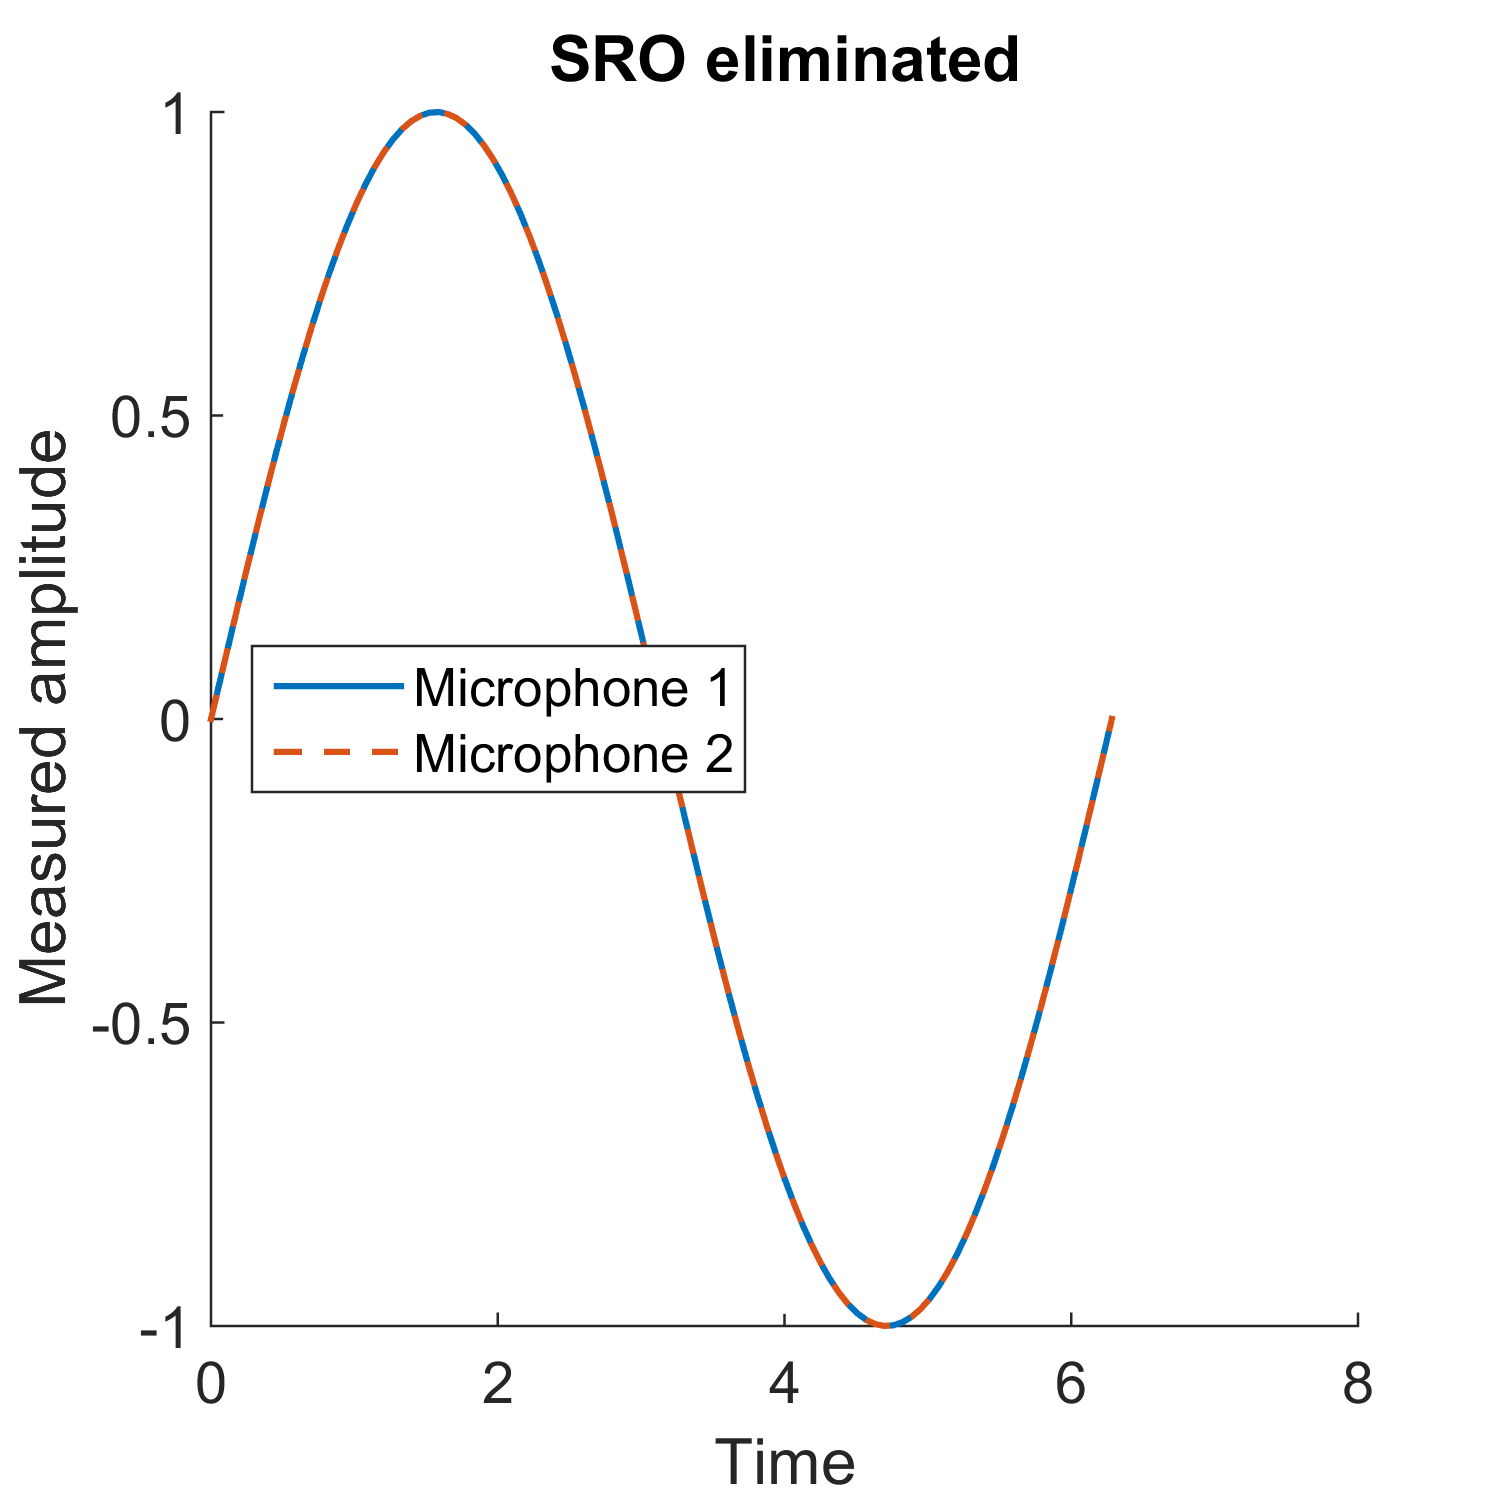
\includegraphics[width=\textwidth]{figures/sro-example/synchronized}
		\caption{TO and SRO have now been eliminated, fully synchronizing the signals.}
		\label{fig:sync-ex3}
	\end{subfigure}
	~
	\begin{subfigure}{0.25\paperwidth}
		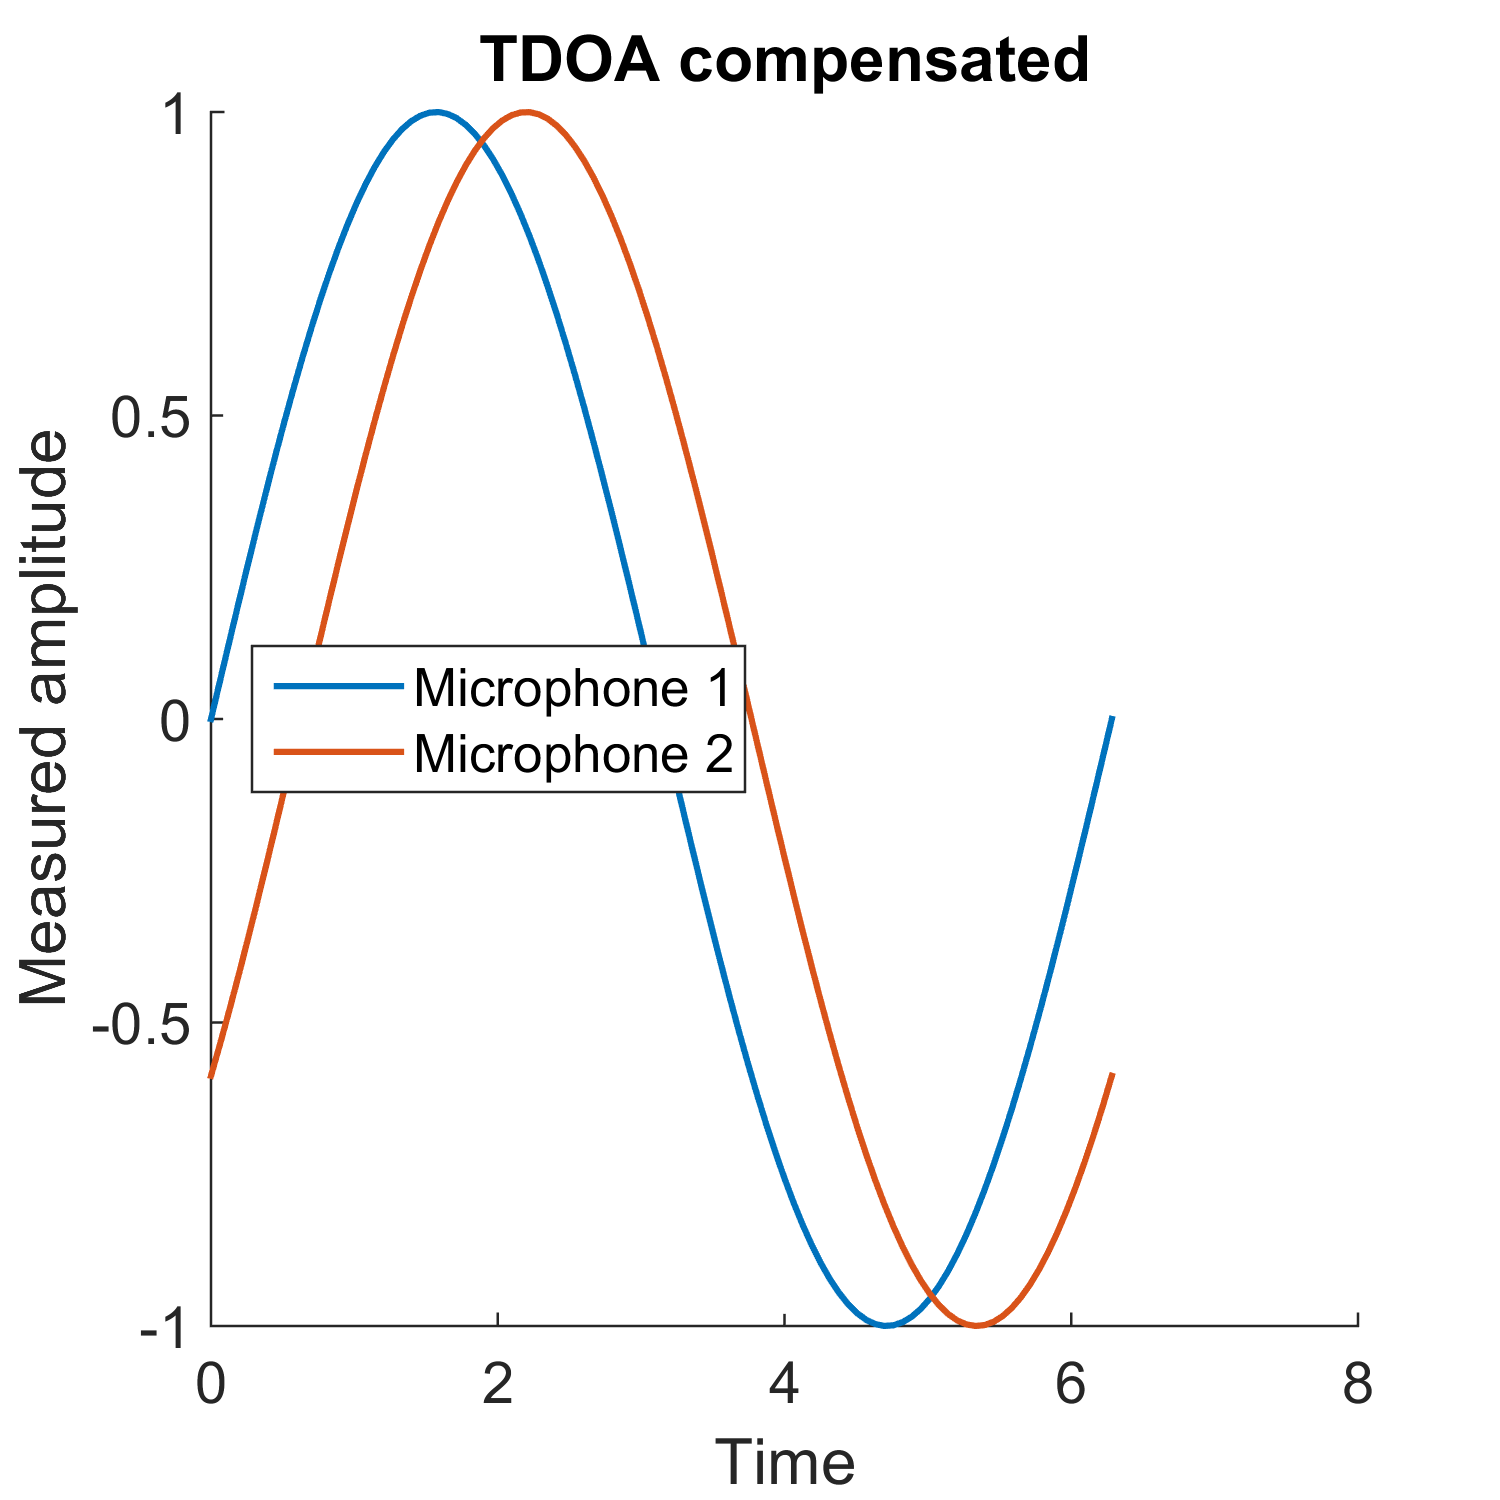
\includegraphics[width=\textwidth]{figures/sro-example/tdoa-compensated}
		\caption{Samples corrected for TDOA from loudspeaker to microphone location.}
		\label{fig:sync-ex4}
	\end{subfigure}
\end{adjustwidth}
\caption[TO and SRO correction stages.]{Example of TO and SRO correction stages.}
\label{fig:synchronization-example}
\end{figure}


\subsection{Time offset}
Formally, the time offset (TO) between two receivers may be described by the following formula \cite{Lasassmeh2010}:
\begin{equation}
\Delta t = \Delta t_{\text{send}} + \Delta t_{\text{access}} +  \Delta t_{\text{prop}} + \Delta t_{\text{receive}}
\end{equation}

In this case, $\Delta t_{\text{send}}$ and $\Delta t_{\text{access}}$ are equal for all smartphones. $\Delta t_{\text{receive}}$ is prone to the random variation associated with audio recording, wireless networking, and processing and $\Delta t_{\text{prop}}$ is due to the propagation time of sound in air.
To correct for TO, the propagation delay and reception delay must both be known; in the first step of synchronization, the sum $\Delta t_{\text{prop}}+\Delta t_{\text{receive}}$ is compensated as exemplified in Fig.~\ref{fig:sync-ex1}-\ref{fig:sync-ex2}. In a second step the propagation delay is added back to the sampled signal, effectively compensating each smartphone for its expected time-difference of arrival (TDOA). This process is illustrated in Fig.~\ref{fig:sync-ex3}-\ref{fig:sync-ex4}.

\subsection{Sampling rate offset}
\label{sec:problem-sro}
The second synchronization requirement is due to clock skew in the individual ADCs used to record audio. Since the ADCs used in smartphones are not typically designed for high-precision sampling, a sampling rate offset (SRO) up to even $10~\mathrm{Hz}$ may be present \cite{pawig2010}. The detrimental influence of sampling rate offset on signal processing performance has been demonstrated by Cherkassky and Gannot \cite{cherkassky2014}.

If left uncompensated, sampling rate offset results in a time offset that changes with time. In order to correct for this, the sample rate offset must be estimated, after which the microphone signals can be resampled to conform to a precise global sample rate \cite{golan2012}.

\paragraph*{}
The following section describes some possible solutions to these two synchronization problems.

\end{document}
